\documentclass[lettersize,journal]{IEEEtran}
\usepackage{amsmath,amsfonts}
\usepackage{algorithmic}
\usepackage{algorithm}
\usepackage{array}
\usepackage[caption=false,font=normalsize,labelfont=sf,textfont=sf]{subfig}
\usepackage{textcomp}
\usepackage{stfloats}
\usepackage{url}
\usepackage{verbatim}
\usepackage{graphicx}
\usepackage{cite}
\hyphenation{op-tical net-works semi-conduc-tor IEEE-Xplore}
% updated with editorial comments 12/2/2022

\begin{document}

\title{Journal DAO: A New Framework for Ownership of Author in Web 3.0}

\author{Tai Jiang,~\IEEEmembership{Follow,~IEEE,}
        % <-this % stops a space
\thanks{Identify applicable funding agency here. If none, delete this.}% <-this % stops a space
\thanks{Manuscript received February 15, 2023; revised February 15, 2023.}}

% The paper headers
\markboth{Journal of \LaTeX\ Class Files,~Vol.~14, No.~8, February~2023}%
{Shell \MakeLowercase{\textit{et al.}}: A Sample Article Using IEEEtran.cls for IEEE Journals}

% \IEEEpubid{0000--0000/00\$00.00~\copyright~2021 IEEE}
% Remember, if you use this you must call \IEEEpubidadjcol in the second
% column for its text to clear the IEEEpubid mark.

\maketitle

\begin{abstract}
Ownership is The most important thing about web 3.0. Using blockchain technology, it is possible to make a paper objectively belong to its author. In the era of centralization, "trust" in an organization is required to complete cooperation, whether it is mutual or intermediary. But decentralized smart contracts allow all collaboration to exist objectively without the need for "trust". Once a paper is published successfully, it is uploaded to the chain using smart contracts. Later, the paper nominally belongs to the author, but actually exists in the database of a website, and once value is created it basically belongs to that website as well. In the framework of decentralized science, the paper no longer exists in the database of a website, but the website goes to map this paper. Each paper creates a decentralized organization that gives a token to the author, the journal, and other interested parties, and once the paper has created value, it is distributed to all holders according to the token.
% 主要强调了拥有
\end{abstract}

\begin{IEEEkeywords}
DAO, smart contract, decentralized autonomous organizations, decentralized funding, decentralized science, DeSci, metaverses, parallel DeSci, parallel intelligence, Web3
\end{IEEEkeywords}

\section{Introduction}
\IEEEPARstart{A}{cademic} publication methods have undergone significant historical transformations, reflecting the evolution of technology, society, and culture.Key trends in the historical evolution of author research publication methods are examined in the flowing.
%学术论文的发表方式在历史上发生了显著的变迁,反映了技术、社会和文化的演进。以下是有关作者发表论文方式的历史变迁的一些主要趋势:
\begin{enumerate}
  \item \textbf{Manuscript Handwriting:} In ancient times, scholars meticulously handwrote academic papers, often by themselves or with the assistance of scribes. These handwritten manuscripts were highly prized and scarce.
  %传统手写和手抄本: 在古代,学术论文通常是手写的,研究者会亲自制作抄本,或者雇佣抄写员来制作。这些手抄本通常是极为珍贵和稀缺的。
  
  \item \textbf{Printing Press Introduction:} The 15th-century Renaissance saw a revolutionary shift with the introduction of the printing press, enabling the mass production and distribution of research, greatly enhancing knowledge accessibility \cite{febvre1997coming}.
  %印刷术的出现: 文艺复兴时期(15世纪)的印刷术革命彻底改变了学术发表的方式。现在,研究者可以使用印刷机来大规模复制和传播他们的研究成果,使知识更容易传播。

  \item \textbf{Academic Journals Emergence:} The late 17th and early 18th centuries marked the rise of academic journals as structured platforms for research dissemination, facilitating the organization and categorization of research findings \cite{willinsky2006access}.
  %学术期刊的兴起: 17世纪末至18世纪初,学术期刊开始兴起,成为学术研究的主要发布渠道。期刊提供了一种有组织的方式,将研究成果分类和发布。

  \item \textbf{Peer Review Inclusion:} The early 20th century brought the prominence of peer review, necessitating expert evaluation of research papers to ensure quality and credibility.
  %同行评审的引入: 20世纪初,同行评审机制开始普及,研究论文需要经过专家同行评审才能被接受发表。这一机制旨在确保研究的质量和可信度。

  \item \textbf{Electronic Journals and Digital Publishing:} The late 20th and early 21st centuries witnessed the transition to electronic journals, providing researchers with online access to publish their papers, significantly increasing research output accessibility and searchability \cite{meadows1997communicating}.
  %电子期刊和数字化发表: 20世纪末至21世纪初,随着互联网的普及,学术期刊逐渐提供了电子版本,研究者可以在线访问和发表论文。数字化发表大大提高了研究成果的可访问性和可搜索性。

  \item \textbf{Open Access Proliferation:} In the 21st century, the open access movement gained momentum, advocating for free public access to research. Open-access journals \cite{swan2012policy} and repositories became more prevalent, promoting knowledge sharing.
  %开放获取运动: 21世纪,开放获取(Open Access)运动兴起,鼓励将研究成果免费对公众开放。开放获取期刊和存档逐渐增多,以提高知识的共享和传播。

  \item \textbf{Preprints Introduction:} Various fields began adopting preprint platforms in which researchers could share their findings before undergoing formal peer review, accelerating research results dissemination.
  % 预印本(Preprints): 一些领域开始采用预印本平台,研究者可以在正式同行评审之前分享他们的研究成果。这缩短了发表过程的时间。

  \item \textbf{Academic Social Media and Blog Utilization:} Scholars increasingly turned to academic social media platforms and blogs to share their research findings, insights, and discussions, expanding their reach and impact.
  %学术社交媒体和博客: 研究者越来越倾向于使用学术社交媒体平台和博客来分享他们的研究成果、见解和讨论,从而扩大了影响力。

  \item \textbf{Blockchain Technology Integration:} Blockchain technology has recently entered academic publishing, offering a decentralized, transparent, and trustworthy publication method, addressing certain traditional publishing challenges \cite{swan2015blockchain} \cite{mougayar2016business}.
  %区块链技术的应用: 区块链技术开始在学术出版领域崭露头角,提供了一种去中心化、透明和可信的发表方式,以解决一些传统出版领域的问题。
\end{enumerate}

This timeline sheds light on the dynamic evolution of research publication methods, continually adapting to new technologies and societal trends. The future of academic publishing is expected to witness further transformations, including expanded open access, increased peer review transparency, enhanced international collaboration, and interdisciplinary research integration. These trends are poised to shape the future of research dissemination.
%这些趋势反映了学术论文发表方式的不断演化,以适应新的技术和社会趋势。未来,学术出版领域可能会继续面临新的变革,例如更广泛的开放获取、更透明的同行评审、更多的国际合作和跨学科研究等。这些趋势有望继续塑造学术发表的未来。

Blockchain is a distributed ledger technology that originally emerged as the foundational technology behind Bitcoin. It employs cryptographic techniques to record data in a series of immutable blocks, forming a chain. The key features of blockchain include decentralization, transparency, security, and immutability, making it a powerful tool applicable to various fields beyond just cryptocurrencies.
%区块链是一种分布式账本技术,最初作为比特币的基础技术而出现。它通过密码学方法将数据记录在一系列不可篡改的区块中,形成一个链。区块链的核心特征包括去中心化、透明性、安全性和不可篡改性。这使其成为一个强大的工具,可用于多种领域,不仅限于加密货币。

Smart contracts are self-executing agreements encoded on a blockchain. They automatically execute, enforce, or verify the terms and conditions of a contract without requiring intermediaries. Smart contracts are code-based and are used for a wide range of applications, from payments to asset management.
%智能合约是区块链上的自动执行合同,其执行受到事先编程的规则和条件的约束。智能合约能够自动执行、验证和执行合同中的条款,无需中介。它们是基于区块链技术的代码,可实现多种应用,从支付到资产管理。

DAO(Decentralized Autonomous Organization) is an organizational structure that operates based on blockchain technology, aiming to achieve automated decision-making and operations without the need for traditional central management. Decision-making in DAOs is conducted through votes by token holders, and rules and processes are encoded by smart contracts rather than central governing authorities. This automated approach enhances transparency, reduces trust-related costs, and provides equal opportunities for community participation\cite{wang2019decentralized}. 
%DAO是一种组织形式,它基于区块链技术,旨在实现自动化决策和运营,无需传统的中央管理。DAO的决策是通过代币持有者的投票进行的,规则和流程是由智能合同编码的,而不是由中央管理机构。这种自动化的方式可以提高透明度、减少信任成本,并为社区参与提供平等的机会。


\textbf{Application of DAO in Article and Journal:}

\begin{itemize}
  \item \textbf{Transparent Peer Review and Publishing Process:} 
  
  Blockchain can be used to create a transparent academic publishing platform, ensuring transparency throughout the peer-review and publishing processes.\cite{nakamoto2008bitcoin} Smart contracts can manage review, publication, and payment procedures, ensuring traceability and fairness.
  %透明的学术出版: 区块链可以用于创建透明的学术出版平台,确保审稿和出版过程的透明性。智能合约可以管理审稿、出版和付款流程,确保可追溯和公平。

  \item \textbf{Protection of Intellectual Property:}
  
  Blockchain and smart contracts can safeguard authors' intellectual property, ensuring their works are not copied or distributed without permission.
  %知识产权保护: 区块链和智能合约可用于保护作者的知识产权,确保其作品不会未经许可就被复制或传播。
  
  \item \textbf{Identity Verification and Reputation Building:} 
  
  Blockchain can be employed to establish scholars' identities and reputations \cite{radziwill2018blockchain}. Smart contracts can automate the validation of scholars' achievements, storing them on the blockchain.
  %身份验证和声誉建立: 区块链可用于建立学者的身份和声誉。智能合约可以自动化验证学者的成就,并将其存储在区块链上。
  
  \item \textbf{Data Sharing and Collaboration:} 
  
  Blockchain and smart contracts can facilitate data sharing and collaboration among scholars, ensuring data integrity and traceability.
  %数据共享和合作: 区块链和智能合约可用于促进学者之间的数据共享和合作,确保数据的完整性和来源可追溯。
  
  \item \textbf{Automated Review and Journal Management:} 
  
  Smart contracts and DAOs can be used to automate review processes and journal management, from reviewer assignments to manuscript evaluations and publication \cite{praitheeshan2019security}.
  %自动化审稿和杂志管理: 智能合约和DAO可以用于自动化审稿流程和杂志管理,从审稿员的分配到稿件的评审和出版。
\end{itemize}

These application examples highlight the potential value of blockchain, smart contracts, and DAO technology in academic publishing and journal management. They enhance transparency, protect intellectual property, verify identity, automate processes, and encourage collaboration. As these technologies continue to evolve, they hold promise for further innovation and efficiency in academia.
%这些应用示例突显了区块链、智能合约和DAO技术在学术出版和杂志管理方面的潜在应用,提高了透明度、知识产权保护、身份验证和自动化审稿流程。随着这些技术的不断发展,它们将有望为学术界提供更多的创新和效率。

This paper emphasizes the transformative impact of DAOs in establishing an explicit ownership of academic research papers by their authors. DAOs empower authors to retain complete control over their works, ensuring that any value generated from these papers is intrinsically linked to the original creators. Through the implementation of DAO, this paper explores the means by which academic papers can be securely attributed to their authors, facilitating a transparent and impartial relationship between the authors and the intellectual assets they produce.
%本文强调了 DAO 在建立作者对其学术研究论文的明确所有权方面的变革性影响。 DAO 使作者能够保留对其作品的完全控制,确保这些论文产生的任何价值都与原始创作者有着内在的联系。通过实施DAO,本文探讨了学术论文可以安全地归属于作者的方法,促进作者与其产生的知识资产之间建立透明和公平的关系

\section{Ownership of Research Data}

This chapter delves into the intricate matter of research data ownership. In the realm of academic research, the question of who possesses, controls, and manages research data is of paramount importance, involving researchers, academic institutions, publishers, and various stakeholders within society. This chapter explores how data ownership impacts academic research, knowledge dissemination, and scientific collaboration. We examine the legal and policy landscape surrounding data ownership in different fields and countries, as well as the management, sharing, and protection of research data. We also investigate existing data-sharing models and open-access policies and their potential effects on the academic community and knowledge innovation. By delving into the issue of research data ownership, we gain a deeper understanding of the challenges and opportunities in today's academic environment, offering new perspectives for future research and collaboration.
%本章将深入探讨论文数据的所有权问题。在学术研究领域,谁拥有、控制和管理研究数据是一个关键议题,涉及到研究人员、学术机构、出版商和社会的各个利益相关方。我们将探讨数据的所有权如何影响学术研究、知识传播和科学合作。此章将考察不同领域和国家对论文数据所有权的法律和政策,以及如何管理、分享和保护研究数据。我们还将研究现有的数据共享模式和开放获取政策,以及它们对学术社区和知识创新的潜在影响。通过深入研究论文数据的所有权问题,我们将更好地理解当前学术环境中的挑战和机遇,为未来的研究和合作提供新的思考。

\begin{figure}[h]
  \centering
  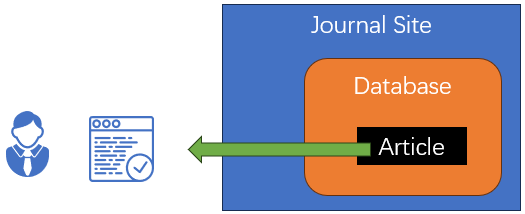
\includegraphics[width=3in]{assets/journalsite.png}
  \caption{Article in Database}
  \label{fig:journalsite}
\end{figure}

From a physical perspective, the data of articles is stored in the database of the journal website (Look at Figure \ref{fig:journalsite}). When regular users access the journal website, they can browse and download articles of interest. The interaction between users and the journal website typically involves the following steps.
%从物理层出发,期刊网站的数据库是文章数据的关键存储点。这些数据库通常位于服务器上,这些服务器可以分布在数据中心或云服务提供商的设施中。当普通用户访问期刊网站时,他们可以通过网络连接访问这些数据库以浏览和下载感兴趣的论文。


\begin{figure}[h]
  \centering
  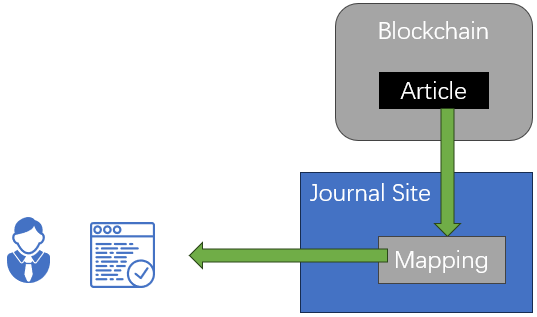
\includegraphics[width=3in]{assets/journalchain.png}
  \caption{Article in Blockchain}
  \label{fig:journalchain}
\end{figure}

When an article is uploaded to a blockchain(Look at Figure \ref{fig:journalchain}), its content, timestamp, and relevant metadata are all recorded on the blockchain. This means that anyone can verify the existence, content, and timestamp of the article. This provides a high level of assurance for the immutability and transparency of documents, particularly with potential significance in research, intellectual property protection, and copyright. Uploading articles to the blockchain also enables decentralized data storage, reducing reliance on centralized institutions. This offers a more open and trustworthy means of data sharing for the academic community and other domains.
%当一篇文章被上链到区块链中,它的内容、时间戳以及相关的元数据都会被记录在区块链上。这意味着任何人都可以验证这篇文章的存在、内容和时间。这为文献的不可篡改性和透明性提供了极高的保障,尤其在科研、知识产权保护和版权方面具有潜在的重要应用。上链文章还可以实现去中心化的数据存储,减少对中央化机构的依赖。这为学术界和其他领域提供了更开放和可信的数据共享方式。


Uploading an article to a blockchain, as compared to storing it in a traditional database, provides the author with a clear and objective ownership of the article. In a traditional database, the ownership of the data and the integrity of the database are controlled by the entity or organization managing the database. Authors and other stakeholders may not have direct control or visibility into the ownership and usage of the data.
%将文章上传至区块链,与将其存储在传统数据库中相比,可以让作者更明确且客观地拥有文章。在传统数据库中,数据的所有权和数据库的完整性由管理数据库的实体或组织控制。作者和其他利益相关方可能无法直接控制或了解数据的所有权和使用情况。

On the other hand, when an article is uploaded to a blockchain, the author can have greater confidence in their ownership and control over the article. The blockchain's decentralized and immutable nature ensures that the ownership records are transparent, tamper-resistant, and not under the sole control of a centralized authority. This empowers authors to have a direct and verifiable claim to their work, which can be particularly important for intellectual property protection, copyright, and ensuring that the author's rights are respected.
%另一方面,当文章上传至区块链时,作者可以更有信心地拥有和控制文章。区块链的去中心化和不可篡改性确保了所有权记录的透明性、防篡改性,并不受中心化权威的独立控制。这使作者能够直接并且可验证地主张他们的作品,这对于知识产权保护、版权以及确保作者的权利得到尊重尤为重要。



\textbf{Compared with traditional journals, articles on the chain belong entirely to the author.}
%相比于传统期刊,链上的文章完全属于作者。


\paragraph{Traditional Databases}
%传统数据库:

Traditional databases are typically controlled by a central entity or organization, with database administrators responsible for management and access control. This centralization may result in less transparent ownership.
%传统数据库通常由中央机构或组织控制,数据库管理员负责管理和授予访问权限。这可能导致数据的所有权不够透明。

Access to and modification of data in traditional databases often depend on access controls set by database administrators. This can lead to disputes or lack of transparency regarding data access.
%数据的访问和修改通常依赖于数据库管理员设置的访问控制。这可能导致对数据访问权限的争议或不透明性。

Data in traditional databases can be relatively easily modified or deleted. This may raise concerns about data security and integrity, especially in cases where intellectual property protection is crucial.
%传统数据库中的数据可以相对容易地被修改或删除。这可能引发数据安全性和完整性的问题,尤其是在需要保护知识产权时。

Ownership and control of data are typically centralized with the database administrator. This centralization introduces a single point of control over data usage, increasing the risk of misuse or improper handling.
%数据的所有权和控制通常集中在数据库的管理者手中。这可能导致对数据使用的单一控制点,增加了数据被滥用或不当处理的风险。

\paragraph{Blockchain}
%区块链:

Every transaction on the blockchain has a clear timestamp, documenting the transfer of ownership. This provides authors with a transparent, immutable record of ownership. Authors can trace ownership back to each stage of the data's lifecycle.
%区块链上的每个交易都有明确的时间戳,记录了数据的所有权转移。这为作者提供了清晰、透明且不可篡改的所有权记录。作者可以追溯到每个阶段数据的所有者。

Blockchain utilizes smart contracts to define and enforce data access permissions. This allows dynamic adjustments of data access rights based on different conditions, such as paid access or specific usage licenses.
%区块链可以使用智能合约来定义和执行数据的使用权限。这使得在不同的条件下,如付费访问或特定使用许可下,可以动态地调整数据的访问权限。

Blockchain is decentralized, with data stored across multiple nodes in the network. This ensures that no single central entity can unilaterally control ownership, enhancing data security and tamper resistance.
%区块链是去中心化的,数据存储在网络的多个节点上。这意味着没有单一的中央机构能够单方面控制数据的所有权,增加了数据的安全性和防篡改性。

Once data is written to the blockchain, it is nearly impossible to modify or delete. This ensures the immutability of data, providing robust protection for the author's rights.
% 一旦数据被写入区块链,几乎不可能对其进行修改或删除。这确保了数据的不可篡改性,作者的权利得到了更强有力的保护。

In summary, blockchain offers a more transparent, immutable, and decentralized ownership mechanism, providing stronger protection for authors' intellectual property and data rights. This is particularly advantageous in scenarios where emphasis is placed on data security, traceability, and transparency.using a blockchain for article storage offers authors a more objective and transparent means of claiming ownership of their work compared to traditional database systems.
%综合而言,区块链提供了更为透明、不可篡改、去中心化的拥有权机制,更好地保护了作者的知识产权和数据权益。这对于需要强调数据的安全性、可追溯性和透明性的应用场景非常有利。使用区块链进行文章存储相对于传统数据库系统,为作者提供了更客观和透明的方式来主张他们的作品所有权

\section{Author Finance from Journal}


In the evolution of electronic journals, websites have become the primary medium for disseminating research papers. Although the content of users' papers remains the intellectual property of the authors, the wealth generated by journals through these papers often belongs predominantly to the journals rather than the authors.
%在电子期刊的发展历程中,论文的载体逐渐从传统的印刷版本过渡到了数字化的网站形式。尽管用户的论文内容仍然属于作者的创作成果,然而,由于现行模式下,杂志通过论文创造的财富往往主要归属于杂志自身,而非作者。

In our hypothetical scenario, we contemplate a shift in this paradigm, envisioning a system where a certain proportion of the generated wealth is allocated back to the authors. Taking paid downloads as a simple example, this mechanism aims to provide authors with a more direct economic incentive. Such a transformation not only has the potential to enhance authors' motivation and creativity but also holds the promise of establishing a more equitable wealth distribution system. This envisioned change could contribute to fostering a sustainable and mutually beneficial development model in the realm of electronic journals, addressing the balance of interests between authors and journals more effectively.
% 在当前设想下,我们可以假设一种改进模式,即按照一定比例将创造的财富回馈给作者。以付费下载为例,这一机制可以为作者提供更直接的经济回报。这种变革不仅有助于激发作者的积极性和创作动力,同时也有望促进更公正的财富分配体系的建立。这样的改变有望在电子期刊领域引入更加可持续和互惠的发展模式,从而更好地满足作者和杂志之间的利益平衡。

\begin{figure}[h]
  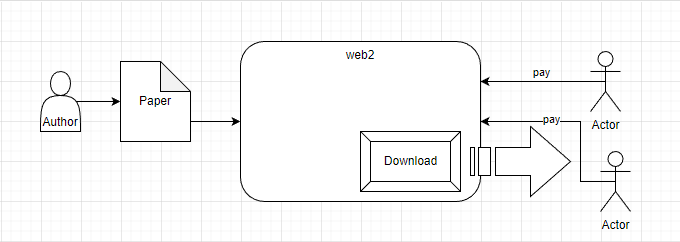
\includegraphics[width=3in]{assets/web2.png}
  \caption{User Pay for Download in Web2.0}
  \label{fig:web2}
\end{figure}

App that enables users to download papers and make money could be designed(Figure \ref{fig:web2}):

\begin{enumerate}
  \item \textbf{Create a platform:} Design an app that provides a platform for users to access academic papers in their field of interest. The app could be designed for PC or Mobile devices(both iOS and Android devices).
  \item \textbf{Build a database:} Build a database of academic papers from various disciplines that can be downloaded by users. You could partner with universities, libraries, and publishers to acquire the papers.
  \item \textbf{Implement a payment system:} Create a payment system that allows users to purchase and download papers. You could charge a fee per paper or offer subscription packages for unlimited access.
  \item \textbf{Integrate social networking features:} Incorporate social networking features such as discussion forums, chat rooms, and rating systems to encourage users to engage with the content and with each other.
  \item \textbf{Create an affiliate program:} Allow users to earn money by referring other users to the app. You could provide a commission for each new user referred, or offer rewards for reaching certain milestones.
  \item \textbf{Implement security measures:} To protect the intellectual property rights of the authors and publishers, implement security measures such as digital rights management (DRM) and watermarking to prevent unauthorized distribution of the papers.
  \item \textbf{Provide customer support:} Ensure that users have access to customer support in case they encounter any issues or have questions. 
\end{enumerate}


Overall, designing an app that enables users to download papers and make money requires careful consideration of legal and ethical issues surrounding academic publishing, as well as the needs and preferences of users. It's important to ensure that the app provides value to both users and content creators, while also operating in a fair and ethical manner.
%总体而言,设计一款使用户能够下载论文并赚钱的应用程序需要仔细考虑围绕学术出版的法律和道德问题,以及用户的需求和偏好。重要的是要确保应用程序为用户和内容创建者提供价值,同时以公平和道德的方式运营。


Web2, also known as the social web, refers to the current state of the internet that we use today, which is primarily focused on social media, e-commerce, and other web-based applications that allow users to interact with each other and with content in various ways. In Web2, payment systems are typically centralized, meaning that they are controlled by a single entity or organization. For example, when we make a purchase on an e-commerce website, we typically use a centralized payment system like PayPal or a credit card. These systems rely on intermediaries to facilitate transactions, which can result in higher transaction fees and longer processing times.
%Web2,也称为社交网络,指的是我们今天使用的互联网的现状,主要集中在社交媒体、电子商务和其他基于网络的应用程序,这些应用程序允许用户相互交互以及与其他人进行交互。内容以多种方式呈现。在 Web2 中,支付系统通常是集中式的,这意味着它们由单个实体或组织控制。例如,当我们在电子商务网站上购物时,我们通常使用 PayPal 或信用卡等集中支付系统。这些系统依赖中介机构来促进交易,这可能会导致更高的交易费用和更长的处理时间。

Web3, also known as the decentralized web, represents a shift toward a more open, decentralized, and secure internet that is built on blockchain technology. In Web3, payment systems are decentralized, meaning that they are not controlled by a single entity or organization. Instead, payments are made using cryptocurrency, which is a digital asset that is secured by cryptographic techniques and operates independently of central banks and other financial institutions. Cryptocurrency payments are processed directly between users without the need for intermediaries, which can result in lower transaction fees and faster processing times.
%Web3,也称为去中心化网络,代表着向基于区块链技术构建的更加开放、去中心化和安全的互联网的转变。在 Web3 中,支付系统是去中心化的,这意味着它们不受单个实体或组织的控制。相反,支付是使用加密货币进行的,加密货币是一种由加密技术保护并独立于中央银行和其他金融机构运作的数字资产。加密货币支付直接在用户之间进行处理,无需中介机构,这可以降低交易费用并缩短处理时间。

\begin{figure}[h]
  \centering
  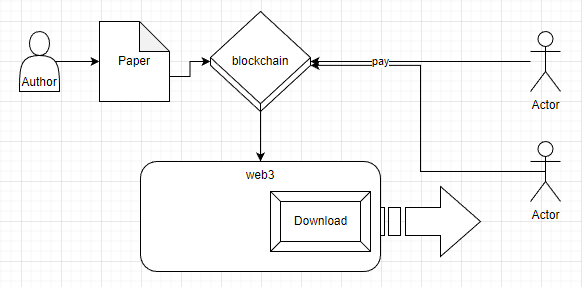
\includegraphics[width=3in]{assets/web3.png}
  \caption{User Pay for Download in Web3.0}
  \label{fig:web3}
\end{figure}


Transforming the app into a DAO framework involves decentralizing control and fostering community involvement. Here's how the app might adapt the design(Figure \ref{fig:web3}):

\begin{enumerate}
  \item \textbf{Decentralize Platform Governance:}
  
  Modify Ownership Structure: Shift ownership and governance to a decentralized autonomous organization (DAO). Token holders in the DAO can participate in decision-making.
  %创建一个平台:设计一个应用,为用户提供访问其感兴趣学术论文的平台。该应用可同时为iOS和Android设备设计。
  \item \textbf{Decentralize Database Building:}
  
  Implement Decentralized Storage: Utilize decentralized storage solutions like IPFS (InterPlanetary File System) to store academic papers in a distributed manner.
  %构建数据库:建立包含各学科学术论文的数据库,用户可下载。您可以与大学、图书馆和出版商合作,获取论文。
  \item  \textbf{Implement Decentralized Payment System:}
  
  Integrate Cryptocurrency Payments: Enable cryptocurrency payments within the DAO for accessing papers. Smart contracts can handle payments, ensuring transparency and security.
  %实施支付系统:创建一个支付系统,允许用户购买和下载论文。您可以按篇收费或提供无限访问的订阅套餐。
  \item \textbf{Decentralize Social Networking Features:}
  
  Token-Based Rewards for Engagement: Reward users with tokens for active participation in discussion forums, chat rooms, and ratings. Token-based systems encourage community engagement.
  %集成社交网络功能:整合社交网络功能,如讨论论坛、聊天室和评级系统,鼓励用户与内容以及其他用户互动。
  \item \textbf{Decentralize Affiliate Program:}
  
  DAO-Based Referral Rewards: Implement a DAO-based referral program where users earn tokens for bringing in new users. Smart contracts can autonomously manage and distribute rewards.
  %创建联盟计划:允许用户通过引荐其他用户到应用赚取奖励。您可以为每位新用户引荐提供佣金,或为达到一定里程碑提供奖励。
  \item \textbf{Implement Security Measures with DAO Consensus:}
  
  Consensus-Driven Security Policies: Let the DAO decide on security measures through consensus. Token holders may vote on and enforce security policies, ensuring community agreement.
  %实施安全措施:为了保护作者和出版商的知识产权,实施数字版权管理(DRM)和水印等安全措施,防止未经授权的论文传播。
  \item \textbf{Customer Support through DAO Governance:}
  
  Community-Driven Support: Establish a community-driven support system where DAO members contribute to resolving issues. This could involve reputation-based systems for trustworthy support.
  %提供客户支持:确保用户可以获得客户支持,以解决问题或提出疑问。
\end{enumerate}

In a DAO framework, decision-making power and platform control are distributed among the community. The integration of blockchain technology and smart contracts ensures transparency, security, and community-driven governance, aligning with the principles of decentralization.
%在 DAO 框架中,决策权和平台控制权分布在社区之间。区块链技术和智能合约的集成确保了透明度、安全性和社区驱动的治理,符合去中心化原则。


Overall, the main difference in payment systems between Web2 and Web3 is the degree of centralization. Web2 payment systems are centralized, while Web3 payment systems are decentralized. While Web3 is still in its early stages, it has the potential to revolutionize the way we think about payments, transactions, and financial systems.
%总体而言,Web2和Web3支付系统的主要区别在于中心化程度。 Web2支付系统是中心化的,而Web3支付系统是去中心化的。虽然 Web3 仍处于早期阶段,但它有潜力彻底改变我们对支付、交易和金融系统的看法。



In the current era of digitization, the act of anchoring a paper on the blockchain signifies the author's complete ownership of the work, opening up boundless possibilities. The introduction of blockchain technology empowers authors with more rights and limitless potential. Once a paper is inscribed on the immutable blockchain, authors not only possess intellectual property rights but also gain absolute control over their creations. This shift in ownership implies that authors can explore innovation more freely, facilitate transparent data sharing, and attain fairer returns from the wealth generated by their works. The immutability and transparency afforded by blockchain provide robust protection for the rights of paper owners, ushering in new possibilities for academic research and knowledge sharing. This profound ownership transformation elevates a paper beyond being merely a conduit for academic dissemination; it becomes a symbol of the unique wealth created by the author, sparking a profound revolution in the relationship between academia and authors.
%在这个时代,随着论文数字化的趋势,将论文上链意味着作者对其作品的彻底拥有。区块链技术的引入赋予了作者更多的权利和无限的可能性。一旦论文被写入不可篡改的区块链,作者不仅仅拥有了知识产权,更获得了对其作品的完全掌控。这样的所有权转变意味着作者可以更自由地探索创新、实现数据的透明共享,并在作品创造的财富中获得更为公平的回报。通过区块链的不可篡改性和透明性,论文的所有者权益得到了更强有力的保障,为学术研究和知识共享带来了新的可能性。这种彻底的拥有使得论文不再仅仅是学术传播的载体,更是作者创造的独特财富的象征,为学术界和作者之间的关系带来了深刻的变革。

  

\section{DAO to DeSci}

The DAO was essentially a smart contract on the Ethereum blockchain that contained a set of rules for how the organization would operate. Members could buy tokens that would give them voting rights to make decisions about which projects to invest in. Once a project was selected, the funds were automatically sent to the project's creators, and the project would be added to the DAO's portfolio.
%DAO 本质上是以太坊区块链上的智能合约,其中包含一组关于该组织如何运作的规则。成员可以购买代币,这将赋予他们投票权,以决定投资哪些项目。一旦选择了项目,资金就会自动发送给项目的创建者,并且该项目将被添加到 DAO 的投资组合中。


\paragraph{Membership and Rights}
In the context of Decentralized Autonomous Governance, the membership and rights of participants are crucial components to ensure the fair operation of the organization or platform. 
%去中心化自治中的成员资格和权利是确保组织或平台公正运作的关键组成部分。

\begin{itemize}
  \item \textbf{Membership:}
  \begin{itemize}
    \item Open Participation: Any eligible individual can join the DAO. This openness ensures broad community involvement, free from geographical or other limitations.
    %开放式参与: 任何符合条件的个体都可以加入去中心化自治的组织。这种开放性确保了广泛的社区参与,不受地域或其他限制。
    \item Equity and Tokens: Membership is often obtained through holding specific tokens or having a certain level of equity. This ensures that members with more significant contributions have greater influence in decision-making.
    %权益和代币: 成员通常通过持有特定的代币或具有一定权益来参与。这确保了对组织贡献较多的成员在决策中拥有更大的影响力。
    \item Community Consensus: Membership may require community consensus, where other members in the community agree to the addition of new members. This can be achieved through mechanisms like voting.
    %社群共识: 成员资格可能需要社群共识,即社区中的其他成员同意新成员的加入。这可以通过投票等机制实现。
  \end{itemize}
  \item \textbf{Member Rights:}
  \begin{itemize}
    \item Proposal Rights: Members have the right to propose actions concerning the organization or platform. Proposals may involve resource allocation, project initiation, rule modifications, etc.
    %提案权: 成员有权提出关于组织或平台行动的提案。提案可以涉及资源分配、项目启动、规则修改等。
    \item Voting Rights: Members have the right to participate in the voting process for proposals. Voting rights are typically correlated with a member's stake or token holdings.
    %投票权: 成员有权参与提案的投票。投票权通常与成员在组织中的权益或代币持有数量相关。
    \item Freedom of Speech: Members have the right to freely express opinions, make suggestions, and engage in discussions within the community. Open communication spaces contribute to the collective decision-making process.
    %言论自由: 成员有权在社区中自由表达意见、提出建议和参与讨论。开放的沟通空间有助于集体决策过程。
    \item Supervision and Audit Rights: Members have the right to oversee the organization's operations and request audits of decision-making and execution processes. Transparency is a fundamental principle in decentralized autonomous governance.
    %监督和审计权: 成员有权监督组织运作,并要求对决策和执行过程进行审计。透明度是去中心化自治的重要原则。
    \item Participation in Community Decisions: Members have the right to participate in community discussions and decision-making processes regarding the organization's strategic direction, rule-making, and other critical decisions.
    %参与社区决策: 成员有权参与关于组织的战略方向、规则制定和其他重要决策的社区讨论和决策过程。
    \item Right to Exit: Members typically have the right to choose to exit the organization. Exiting may involve specific processes and conditions to ensure fairness and transparency.
    %退出权: 成员通常有权选择退出组织。退出可能会涉及特定流程和条件,以确保公平和透明。
  \end{itemize}
\end{itemize}

The design of membership and rights aims to balance individual autonomy with the interests of the overall community, ensuring fairness and stability in decentralized autonomous governance systems. This balance contributes to creating an open, transparent, and sustainable community governance model.
%成员资格和权利的设计旨在平衡个体自主性和整体社区的利益,确保去中心化自治系统的公正性和稳定性。这种平衡有助于创造一个开放、透明和具有可持续性的社区治理模型。

\paragraph{Proposal and Voting}
In the framework of a DAO, the proposal and voting mechanisms play a pivotal role in facilitating collective decision-making among its members:
%在去中心化组织(DAO)的框架中,提案和投票是成员共同参与组织决策的关键组成部分

\begin{itemize}
  \item \textbf{Proposal:}
  \begin{itemize}
    \item Submission of Proposals: Any member of the DAO has the right to propose actions for the organization, which can include decisions related to fund allocation, strategic directions, or proposals for new projects.
    %提交提案: 任何DAO成员都有权提出关于组织行动的提案,这可以是关于资金分配、战略方向、新项目的提议等。
    \item Content of Proposals: Proposals should provide a clear outline of their purpose, implementation plan, required resources, etc., enabling members to have a comprehensive understanding of the proposal's content.
    %提案内容: 提案应该清晰说明其目的、执行计划、所需资源等,以便成员全面了解提案的内容
    \item Smart Contract Execution: Proposals are typically defined by smart contracts to ensure that their execution follows established rules without the need for central control.
    %智能合约执行: 提案通常由智能合约定义,确保提案的执行按照规则进行,无需中央控制。
  \end{itemize}
  \item \textbf{Voting:}
  \begin{itemize}
    \item Voting Rights: Members acquire voting rights based on their stake in the DAO (which could be the quantity of tokens held or other contribution metrics).
    %投票权: 成员根据其在DAO中的权益(可能是持有的代币数量或其他贡献度量)获得相应的投票权。
    \item Voting Mechanism: Various voting mechanisms can be employed, such as one member, one vote, or token-weighted voting, depending on the DAO's design.
    %投票方式: 投票可以采用不同的机制,如一人一票、代币投票等,具体规则取决于DAO的设计。
    \item Transparency and Immutability: The voting process is recorded on the blockchain, ensuring transparency and immutability, allowing anyone to verify the voting results.
    %透明度和不可篡改性: 投票过程被记录在区块链上,确保透明度和不可篡改性,任何人都可以验证投票结果。
  \end{itemize}
  \item \textbf{Voting Results:}
  \begin{itemize}
    \item Decision-Making: Proposals need to garner sufficient support through votes to be accepted. Typically, reaching or surpassing a predetermined threshold triggers the execution of the proposal.
    %决策达成: 提案需要获得足够多的支持票数才能通过。通常,达到或超过预定的门槛值会触发提案的执行
    \item Smart Contract Execution: Once a proposal is approved, related smart contracts automatically execute the actions outlined in the proposal, such as fund allocation or changing the organization's state.
    %智能合约执行: 一旦提案获得通过,相关的智能合约会自动执行提案中规定的行动,例如分配资金或改变组织的状态。
  \end{itemize}
\end{itemize}

The proposal and voting mechanisms enable a decentralized and democratic governance process within a DAO. Each member has equal participation rights, and the transparency and auditability of voting results contribute to ensuring fairness and credibility in organizational decision-making. This design philosophy aims to eliminate centralized authority, fostering collective participation of DAO members in shaping the organization's future.
%提案和投票机制使得DAO的治理过程变得去中心化且民主。每个成员都有平等的参与权,并且投票结果是透明可审计的,这有助于确保组织决策的公正性和可信度。这一设计理念旨在消除中心化的权威,并使DAO成员共同参与决策,塑造组织的未来发展。


After the author submits the paper, they enter the DAO framework, and tokens are allocated to both the publisher and the author according to a predetermined ratio. This process signifies the integration of DAO principles into the academic publishing workflow.
%作者提交论文之后,即可进入DAO框架,并且按照一定比重分配给出版商和作者相应的代币。这一过程标志着将去中心化自治组织(DAO)原则融入学术出版流程中。

\begin{figure}[h]
  \centering
  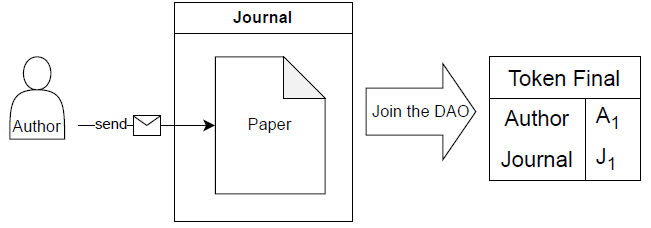
\includegraphics[width=3.2in]{assets/daopaper.png}
  \caption{Distribute Token by DAO}
  \label{fig:distributetoken}
\end{figure}

Figure \ref{fig:distributetoken} is the process:
%以下是该过程的详细步骤:

\begin{enumerate}
  \item Author Submission: The author submits their paper to the DAO-powered academic publishing platform.
  %作者将论文提交给DAO驱动的学术出版平台。
  \item Token Allocation: Tokens are allocated to the author and the publisher. Tokens can be utilized within the DAO ecosystem. 
  %代币分配: 作者和出版商分配代币。代币可以在DAO生态系统中使用。
  \item Community Governance: DAO members, including authors and publishers, may participate in governance decisions related to the platform. 
  %社区治理: DAO成员,包括作者和出版商,可以参与与平台相关的治理决策。
\end{enumerate}


\begin{figure}[h]
  \centering
  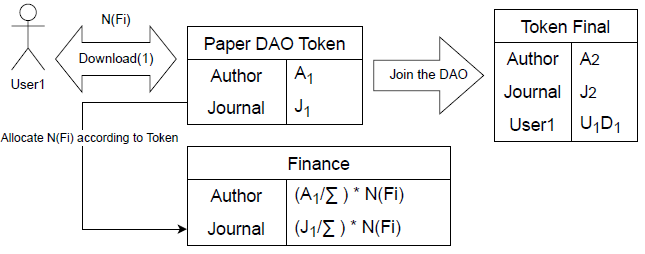
\includegraphics[width=3.2in]{assets/download1.png}
  \caption{Distribute Token while User Download}
  \label{fig:financetoken}
\end{figure}

Figure \ref{fig:financetoken} is the process: When a user creates a financial activity, such as paid downloads, rewards are distributed to all holders based on their previous token holdings. Additionally, the user who creating the financial activity receives a certain amount of tokens as a reward for their contribution, becoming a new holder.
%当用户创造了一项财务活动(例如付费下载),根据之前的代币持有情况,将奖励分配给所有持有者。同时,这个用户也会因为其贡献而获得一定数量的代币,成为新的持有者。


\begin{figure}[h]
  \centering
  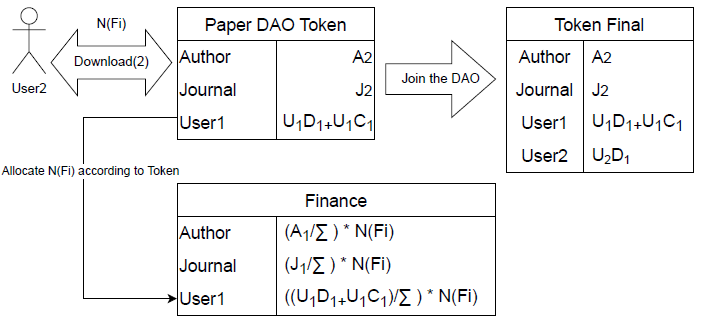
\includegraphics[width=3.2in]{assets/donwload2.png}
  \caption{Distribute Token while Another User Download}
  \label{fig:financetoken2}
\end{figure}

Figure \ref{fig:financetoken2} is the process when another user makes a paid download, the finance generated will be distributed among the author, publisher, and user1 based on their token holdings. Subsequently, user2 will also become a new token holder as a result of their contribution.
%当另外一个用户付费下载,所生成的财务将根据其代币持有量分配给作者、发行商和用户1。随后,用户2也将因其贡献而成为新的代币持有者。

After voluntarily making a payment, users' ability to participate contributes to a robust incentive mechanism, fostering a sense of autonomy within the entire framework. Through this design, users become direct contributors to financial activities, injecting new value into the framework and creating potential opportunities for self-reward. This decentralized autonomous model empowers users to engage directly in decision-making and contributions, shaping a more open, fair, and virtuous ecosystem. Overall, this autonomous framework cultivates a more positive and sustainable participation experience for users and the entire community.
%用户自主付费后,其参与框架的能力构成了一种积极的激励机制,为整个系统的自治性提供了有力支持。通过这一设计,用户成为财务活动的直接贡献者,其行为不仅为框架注入了新的价值,同时也为自身创造了潜在的奖励机会。这种去中心化的自治模式使得用户能够更加直接地参与决策和贡献,从而塑造了一个更加开放、公正、而且具有良性循环的生态系统。整体而言,这种自治的框架为用户和整个社区创造了更为积极和可持续的参与体验。

Once the paper is on the blockchain, it unequivocally belongs to the author, author is the real owner,that creating endless possibilities, especially in terms of financial activities. This means that the author not only owns their work but can also leverage blockchain technology to create various financial opportunities. Authors can receive rewards through financial activities, which may include paid downloads, knowledge exchanges, collaborative projects, and more. This decentralized framework provides authors with greater creative freedom and potential economic returns, enabling them to be more independent and influential in the academic domain. Overall, putting a paper on the blockchain opens up a new and forward-thinking path for authors.
%论文一旦上链,将完全归属于作者,作者就是真正的拥有者,为作者创造了无限的可能性,特别是在财务活动方面。这意味着作者不仅拥有其作品的所有权,而且可以利用区块链技术创造各种财务机会。作者可以通过财务活动获得回报,这可能包括付费下载、知识交流、合作项目等。这种去中心化的框架为作者提供了更大的创作自由和潜在的经济回报,使其在学术领域更加独立和有影响力。整体而言,论文上链为作者开辟了一个全新的、具有前瞻性的创作道路。

\section{Conclusion}
This paper extensively explores the framework of Decentralized Autonomous Organizations (DAOs) and provides a thorough analysis of its potential applications in the academic publishing domain. By placing papers on the blockchain, we have achieved transparency in ownership, allowing authors to have complete control over their works while also creating diverse financial opportunities. The autonomous nature of DAO enables users to directly participate in decision-making and contributions, constructing an ecosystem that is open, fair, and characterized by positive feedback loops.
%本文深入探讨了去中心化自治组织(DAO)的框架,并就其在学术出版领域的潜在应用进行了详尽分析。通过将论文上链,我们实现了论文所有权的透明化,使作者能够完全拥有其作品,同时也为其创造了丰富的财务机会。DAO的自治性质使得用户能够直接参与决策和贡献,构建了一个开放、公正、具有良性循环的生态系统。

DAOs have several advantages over traditional organizations, such as:

\begin{itemize}
\item{Lower costs: DAOs eliminate the need for intermediaries, lawyers, accountants, or managers, reducing the overhead and bureaucracy involved in running an organization.}
%降低成本:DAO 消除了对中介机构、律师、会计师或经理的需求,减少了组织运营所涉及的管理费用和官僚作风。
\item{Higher efficiency: DAOs enable faster and more accurate decision-making, as well as automated execution of tasks and transactions.}
%更高的效率:DAO 可以实现更快、更准确的决策,以及任务和交易的自动执行
\item{Greater innovation: DAOs foster a culture of experimentation and creativity, as anyone can propose and contribute to new ideas or initiatives.}
%更大的创新:DAO 培养了一种实验和创造力的文化,因为任何人都可以提出新的想法或举措并为其做出贡献。
\item{Enhanced security: DAOs are protected by cryptography and consensus mechanisms, making them immune to hacking, fraud, or manipulation.}
%增强的安全性:DAO 受到密码学和共识机制的保护,使其免受黑客、欺诈或操纵的影响。
\item{Increased inclusivity: DAOs are open and accessible to anyone who shares the vision and values of the organization, regardless of their location, background, or status.}
%增强包容性:DAO 是开放的,任何与组织有共同愿景和价值观的人都可以使用,无论其位置、背景或地位如何。
\end{itemize}

DAOs are not without challenges, however. Some of the main challenges include:

\begin{itemize}
\item{Legal uncertainty: DAOs operate in a gray area of the law, as they do not fit into existing legal frameworks or jurisdictions. This creates risks and liabilities for the participants and the beneficiaries of the DAO.}
%法律不确定性:DAO 在法律的灰色地带运作,因为它们不符合现有的法律框架或司法管辖区。这给 DAO 的参与者和受益人带来了风险和责任。
\item{Ethical dilemmas: DAOs may face ethical issues or conflicts of interest, as they may not align with the moral values or social norms of the wider society.}
%道德困境:DAO 可能面临道德问题或利益冲突,因为它们可能与更广泛社会的道德价值观或社会规范不一致
\item{Technical complexity: DAOs rely on complex and experimental technologies, such as blockchain and smart contracts, which may have bugs, vulnerabilities, or unforeseen consequences.}
%技术复杂性:DAO 依赖于复杂的实验性技术,例如区块链和智能合约,这些技术可能存在错误、漏洞或不可预见的后果。
\item{Governance issues: DAOs may struggle to achieve consensus, resolve disputes, or adapt to changing circumstances, as they lack a clear leadership or authority structure.}
\end{itemize}
%治理问题:由于缺乏明确的领导或权力结构,DAO 可能难以达成共识、解决争端或适应不断变化的环境。

In summary, Decentralized Autonomous Organizations inject new vitality into academic publishing, creating a more equitable environment for both authors and readers. This innovative model holds promise for paving new paths in the development of academia, fostering the free dissemination and sharing of knowledge.
%综上所述,去中心化自治组织为学术出版注入了新的活力,为作者和用户创造了更加公平和有利的环境。这一创新模式有望为学术界的发展开辟新的道路,促进知识的自由传播和共享。

% \section*{Acknowledgments}
% This should be a simple paragraph before the References to thank those individuals and institutions who have supported your work on this article.



% {\appendix[Proof of the Zonklar Equations]
% Use $\backslash${\tt{appendix}} if you have a single appendix:
% Do not use $\backslash${\tt{section}} anymore after $\backslash${\tt{appendix}}, only $\backslash${\tt{section*}}.
% If you have multiple appendixes use $\backslash${\tt{appendices}} then use $\backslash${\tt{section}} to start each appendix.
% You must declare a $\backslash${\tt{section}} before using any $\backslash${\tt{subsection}} or using $\backslash${\tt{label}} ($\backslash${\tt{appendices}} by itself
%  starts a section numbered zero.)}



%{\appendices
%\section*{Proof of the First Zonklar Equation}
%Appendix one text goes here.
% You can choose not to have a title for an appendix if you want by leaving the argument blank
%\section*{Proof of the Second Zonklar Equation}
%Appendix two text goes here.}




\bibliography{refs}
\bibliographystyle{IEEEtran}


\newpage

\section{Biography Section}
If you have an EPS/PDF photo (graphicx package needed), extra braces are
 needed around the contents of the optional argument to biography to prevent
 the LaTeX parser from getting confused when it sees the complicated
 $\backslash${\tt{includegraphics}} command within an optional argument. (You can create
 your own custom macro containing the $\backslash${\tt{includegraphics}} command to make things
 simpler here.)
 
\vspace{11pt}

\bf{If you include a photo:}\vspace{-33pt}
\begin{IEEEbiography}[{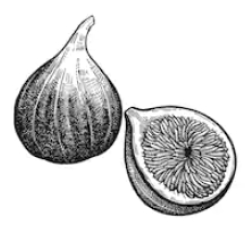
\includegraphics[width=1in,height=1.25in,clip,keepaspectratio]{fig1}}]{Michael Shell}
Use $\backslash${\tt{begin\{IEEEbiography\}}} and then for the 1st argument use $\backslash${\tt{includegraphics}} to declare and link the author photo.
Use the author name as the 3rd argument followed by the biography text.
\end{IEEEbiography}

\vspace{11pt}

\bf{If you will not include a photo:}\vspace{-33pt}
\begin{IEEEbiographynophoto}{John Doe}
Use $\backslash${\tt{begin\{IEEEbiographynophoto\}}} and the author name as the argument followed by the biography text.
\end{IEEEbiographynophoto}




\vfill

\end{document}


